\section{Introduction}
\label{sec:intro} 
\begin{figure}[t]
  \centering
  % Top Image: The AI Brain
  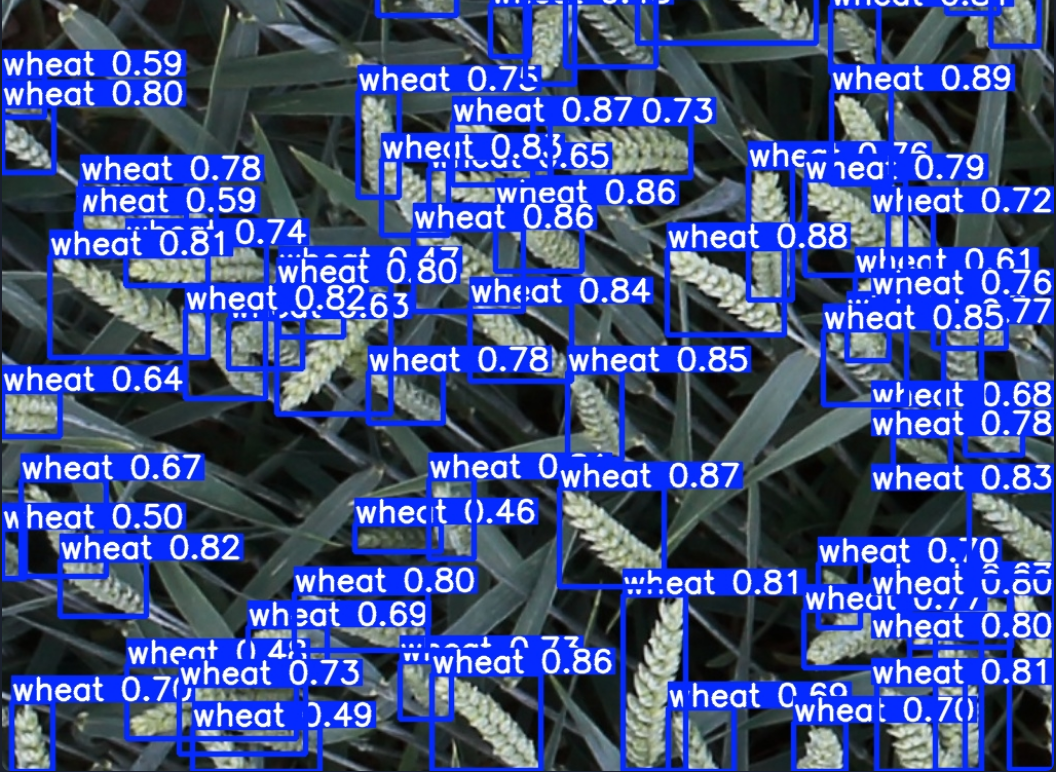
\includegraphics[width=\linewidth]{sec/teaser_wheat_only.png}\\
  \vspace{2mm} 
  % Bottom Image: The Business Logic
  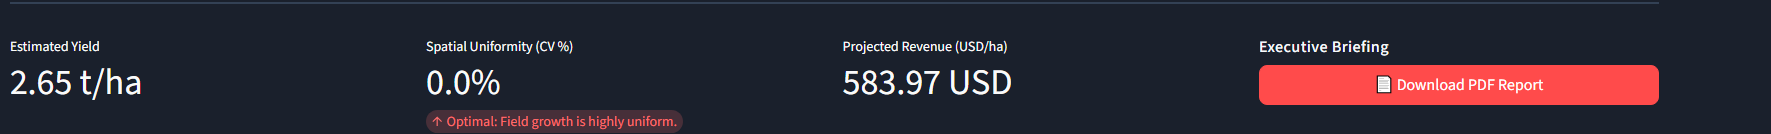
\includegraphics[width=\linewidth]{sec/teaser_statistic.png}
  
  \caption{The AgriVision pipeline. \textbf{Top:} The YOLOv8s architecture successfully extracts features in dense, occluded field topologies. \textbf{Bottom:} The deterministic agronomic engine translates bounding box data into localized metrics ($t/ha$ and CV\%) with automated executive reporting.}
  \label{fig:teaser}
\end{figure}

The optimization of agricultural productivity is a critical pillar of global food security. As climate change and resource depletion accelerate, the necessity for precise, scalable, and automated yield estimation has become a fundamental survival requirement \cite{fao2023}. Wheat (\textit{Triticum aestivum}) represents a primary source of global caloric intake, yet in many developing nations, the agricultural pipeline remains bottlenecked by intensive manual labor. Automating the mechanical analysis of crop yields not only reduces the margin of human error but actively reallocates human capital toward strategic agronomic development and resource management.

Despite the rapid integration of Unmanned Aerial Vehicles (UAVs) in modern agriculture, a significant technical gap remains. Current systems are highly fragmented; they often provide rudimentary computer vision for wheat head detection but fail to translate those spatial coordinates into actionable business intelligence. Relying strictly on bounding boxes without a secondary analytical engine leaves farmers to manually interpret the data, effectively defeating the purpose of automation. 

To resolve this fragmentation, we introduce the AgriVision Decision Support System: an end-to-end, deep learning pipeline designed to seamlessly convert raw drone imagery into localized statistical insights. Our system leverages a custom-tuned YOLOv8 small (YOLOv8s) architecture, specifically optimized on the Global Wheat Detection dataset \cite{existing_study1}, to generate tight bounding boxes around wheat heads even in dense, occluded field topologies. 

Beyond strict detection, the core value proposition of AgriVision is its deterministic agronomic engine. Our architecture processes batch inputs of high-resolution UAV imagery and autonomously computes critical field metrics, including crop spatial variance (health uniformity) and yield estimations measured in tons per hectare ($t/ha$). Furthermore, the engine features dynamic localization, supporting automated configurations for 10 distinct national agronomic profiles, alongside custom parameterization for specialized fields. By bridging the gap between pixel-level detection and macro-level analytics, this system offers a highly scalable, low-friction solution for next-generation digital agriculture.
